\section{Taschenrechner}

\flushleft

\begin{minipage}{0.49\textwidth}
Implementiere das Klassendiagramm rechts mit Hilfe von Blockly. Probiere deine Methode aus (siehe Anleitung auf der Vorderseite). Fülle die Lücken im Java-Code unten aus, wenn deine Methoden funktionieren.
\end{minipage}
\hfill
\begin{minipage}{0.49\textwidth}
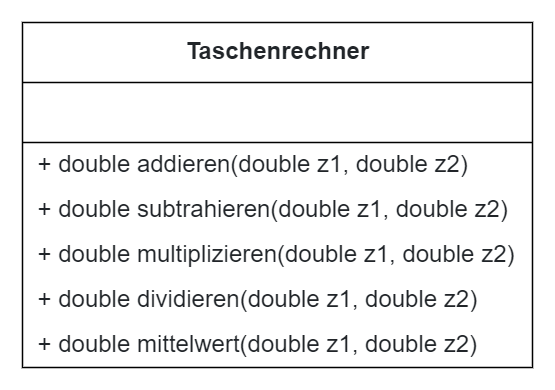
\includegraphics[width=\linewidth]{_Aufgaben/BlocksAndJava/img/Taschenrechner.png}
\end{minipage}

\LARGE


\begin{lstlisting}[escapechar=\&]

public class Taschenrechner
{    
    public & \LoesungLuecke{double addieren(double z1, double z2) \{ }{12cm} &
        
            & \LoesungLuecke{return z1 + z2;}{12cm} &
    }
    public &\LoesungLuecke{double subtrahieren(double z1, double z2) \{ }{12cm}&
        
            & \LoesungLuecke{return z1 - z2;}{12cm} &
    }
    public &\LoesungLuecke{double multiplizieren(double z1, double z2) \{ }{12cm}&
        
            & \LoesungLuecke{return z1 * z2;}{12cm} &
    }
    public & \LoesungLuecke{double dividieren(double z1, double z2) \{ }{12cm}&
        
            & \LoesungLuecke{return z1 + z2;}{12cm} &
    }
    public & \LoesungLuecke{double mittelwert(double z1, double z2) \{ }{12cm} &
        
            & \LoesungLuecke{return (z1 + z2) / 2;}{12cm} &
    }
}
\end{lstlisting}